\section{Obiettivi}

\begin{itemize}
    \item Comprendere lo spazio di indirizzamento virtuale
    \item Conoscere la differenza tra stack e heap
    \item Saper spiegare perché i puntatori sono pericolosi
    \item Conoscere quali bug tipici nascono in C/C++
    \item Spiegare perché Rust introduce i concetti di possesso, prestito, smart pointer
\end{itemize}

\section{Perché studiare come è organizzata la memoria?  }

90\% dei bug di sistema  $\rightarrow$ Accessi illeciti alla memoria o mancata sincronizzazione in programmi concorrenti.

Rust offre una risposta a questi problemi

\begin{minted}[breaklines]{c}
int* p = (int*)malloc(sizeof(int)); 
free(p); 
*p = 5; // cosa succede? 
\end{minted}

\section{Programmi e loro esecuzione  }

Un programma eseguibile è costituito da un insieme di istruzioni macchina, dati, valori di configurazione e controllo rappresentati come sequenze di numeri binari.
Il significato delle istruzioni macchina è cablato all'interno del processore specifico per cui il programma è stato creato.
Il significato delle informazioni restanti è contenuto, in parte, nelle istruzioni macchina e, per la parte restante, dipende dal sistema operativo (se c'è) o da particolari caratteristiche del processore stesso.\newline

Per poter essere eseguito, un programma deve essere caricato all'interno della memoria accessibile al processore. 
\begin{itemize}
    \item Nei sistemi più piccoli (es., Arduino) questo avviene grazie ad hardware specifico che memorizza in modo semi-permanente quanto necessario nella memoria flash.
    \item Nei sistemi più grandi, un modulo del sistema operativo (\textbf{loader}) si occupa di trasferire dal disco alla memoria RAM il contenuto del file eseguibile
\end{itemize}

Una volta che il programma è presente in memoria, può essere eseguito. Il processore preleva dalla memoria, una alla volta, le istruzioni macchina del programma e provvede ad eseguirle. 


L'esecuzione di un'istruzione determina quali effetti collaterali debbano avvenire e quale debba essere la prossima istruzione da eseguire. Modifiche nelle informazioni contenute nel processore stesso e/o nella memoria. Eventuali interazioni con altre periferiche collegate al processore stesso (I/O). \newline

Il modello base di esecuzione prevede l'alternarsi continuo di tre fasi:

\begin{itemize}
    \item Fetch - Un'istruzione viene trasferita dalla memoria all'interno del processore
    \item Decode - L'istruzione prelevata viene trasformata in comandi da eseguire
    \item Execute - I comandi vengono eseguiti
\end{itemize}




\section{Spazio di indirizzamento  }

L’esecuzione di un programma avviene nel suo \textbf{spazio di indirizzamento.} Sottoinsieme delle celle indirizzabili, gestito dal sistema operativo. Dati, istruzioni, informazioni di controllo, … sono memorizzati come valori al suo interno. 
Lo spazio di indirizzamento può essere immaginato come un enorme array di byte, che possono essere letti individualmente, a coppie, a gruppi di 4, 8 alla volta, in base al parallelismo del processore (8, 16, 32 o 64 bit).


Il numero di celle \textbf{potenzialmente} presenti nello spazio di indirizzamento dipende dal processore. Il numero di celle \textbf{effettivamente} presenti, è limitato dalla quantità di RAM disponibile ed è controllato dal sistema operativo.

Nel caso di CPU Intel x64, il processore opera a 64 bit. Ma lo spazio di indirizzamento si estende tra $0$ e $2^{48}-1$(scelta di implementazione).
All'interno di questo, però, solo una piccola parte di indirizzi è effettivamente presente.\newline

Gli indirizzi che un programma utilizza non corrispondono - in generale - all'effettiva posizione che un dato assume in memoria  

\begin{itemize}
    \item Il codice fa riferimento ad \textbf{indirizzi virtuali}
    \item L'hardware utilizza \textbf{indirizzi fisici}
\end{itemize}


Un apposito blocco hardware presente nel processore (\textbf{MMU - Memory Management Unit}) si occupa di tradurre l'indirizzo virtuale in indirizzo fisico.

Tale traduzione garantisce che:

\begin{itemize}
    \item Programmi diversi contemporaneamente in esecuzione non possano interferire tra loro
    \item Consente di controllare quali operazioni siano possibili (lettura, scrittura, esecuzione)
    \item Permette inoltre di scrivere programmi che manipolano dati più grossi della memoria fisica effettivamente presente
\end{itemize}



\begin{figure}
    \centering
    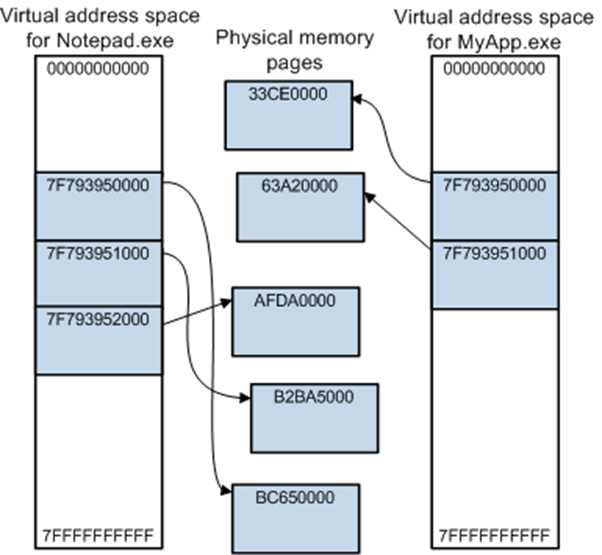
\includegraphics[width=0.75\linewidth]{images/API_Programming/Memoria/Memoria-esempio7.png}
\end{figure}



\section{Effetti pratici  }
\begin{itemize}
    \item Segmentation fault
        \begin{itemize}
            \item Tentativo di accedere ad indirizzo non mappato o senza gli adeguati permessi
            \item Il processore blocca l'esecuzione e rimanda al sistema operativo (che termina brutalmente il
            \item programma)
        \end{itemize}
    \item Page fault
        \begin{itemize}
            \item Tentativo di accedere ad un indirizzo appartenente ad un blocco il cui contenuto è stato salvato su disco
            \item Il processore richiede l'intervento del sistema operativo che ricerca una pagina fisica libera e vi trasferisce il contenuto del blocco presente nel file di paginazione
            \item Al termine il processore ritenta l'accesso e procede normalmente
        \end{itemize}
    \item Trashing
        \begin{itemize}
            \item Se il programma cerca di accedere rapidamente ad una grande quantità di dati paginati, il sistema passa più  tempo a spostare pagine tra disco e memoria fisica di quanto ne possa dedicare all'esecuzione vera e propria
        \end{itemize}
\end{itemize}


\section{Gerarchia di memoria  }

Nei sistemi non elementari, il processore \textbf{non legge/scrive} direttamente dalla memoria RAM. Tra i due elementi viene interposta la memoria \textbf{cache}. Questa ha il compito di velocizzare l'accesso alle informazioni cercando di anticipare il bisogno di informazioni da parte della CPU.

Si basa sul \textbf{principio di località} dei programmi: se è stato appena fatto accesso all'indirizzo I, è molto probabile che venga fatto subito dopo accesso all'indirizzo $I + \Delta$ (con $\Delta$ molto piccolo).

La memoria cache si basa su dispositivi il cui tempo di accesso è molto più rapido di quello offerto dalla memoria RAM tradizionale, ma dotati di una capacità molto inferiore (pochi KB/MB).

Per questo Vec<T> è quasi sempre meglio di LinkedList<T>
\section{Località }

\begin{figure}
    \centering
    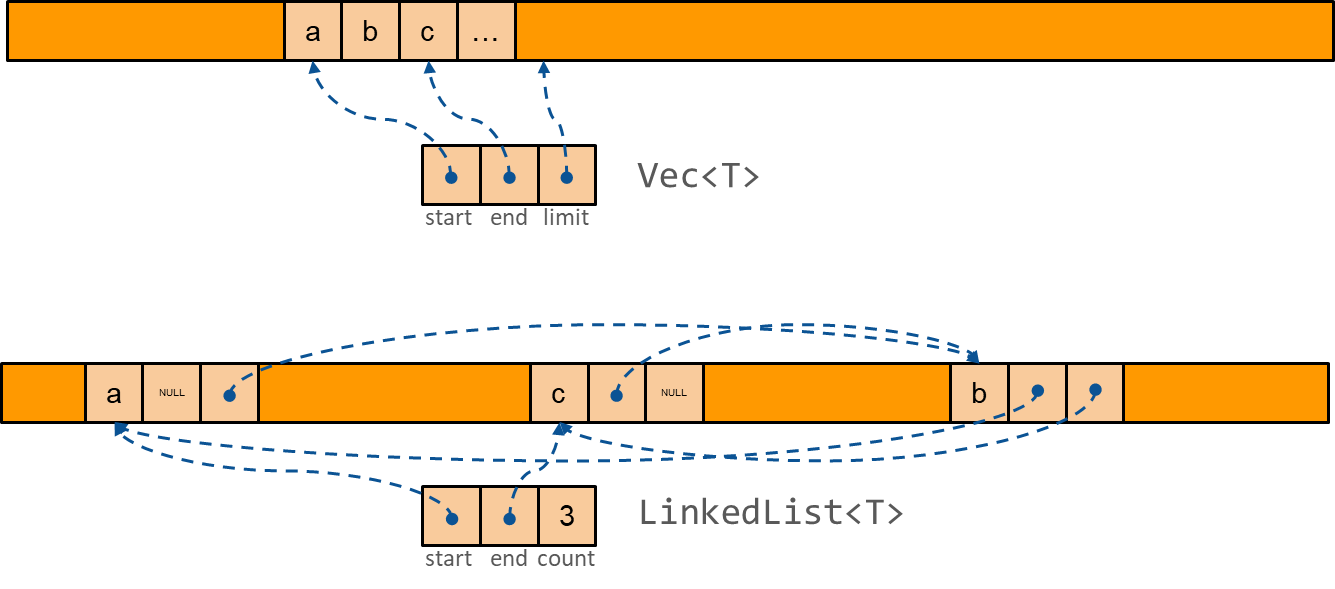
\includegraphics[width=0.75\linewidth]{images/API_Programming/Memoria/Memoria-esempio6.png}
\end{figure}

\section{Esecuzione e programmi di alto livello  }

Utilizzando linguaggi di programmazione ad alto livello, i dettagli legati al meccanismo di esecuzione sono normalmente invisibili.

Tuttavia, per poter garantire il livello di astrazione necessario, essi devono introdurre delle sovrastrutture che impattano sul codice che viene scritto dal programmatore…e introducono un insieme di \textbf{vincoli} e \textbf{restrizioni} di cui è necessario essere pienamente coscienti.

\section{Modello di esecuzione di un programma}

Ogni linguaggio di programmazione propone uno specifico modello di esecuzione, un insieme di comportamenti che attuati dall'elaboratore a fronte dei costrutti di alto livello del linguaggio.


Tale modello per lo più non corrisponde a quello di un dispositivo reale, come fa il processore ad eseguire solo Fatch, Decode ed Execute? Utilizzando strutture dati intermedie e da un insieme di run-time library. 
È compito del compilatore introdurre uno strato di adattamento che implementi il modello nei
termini offerti dal dispositivo soggiacente.

Questo strato è composto, da un lato, da una specifica modalità di traduzione dei costrutti di alto
livello in istruzioni macchina e, dall'altro, da un insieme di funzionalità di supporto offerte sotto forma
di libreria di supporto all'esecuzione (run-time library).

\section{Livelli di astrazione}
La compilazione trasforma il programma sorgente in un nuovo programma dotato di
un modello di esecuzione ed un insieme di istruzioni più semplice. Che può essere eseguito da una macchina fisica (CPU) o subire un'ulteriore trasformazione (esecuzione virtuale)

\begin{figure}
    \centering
    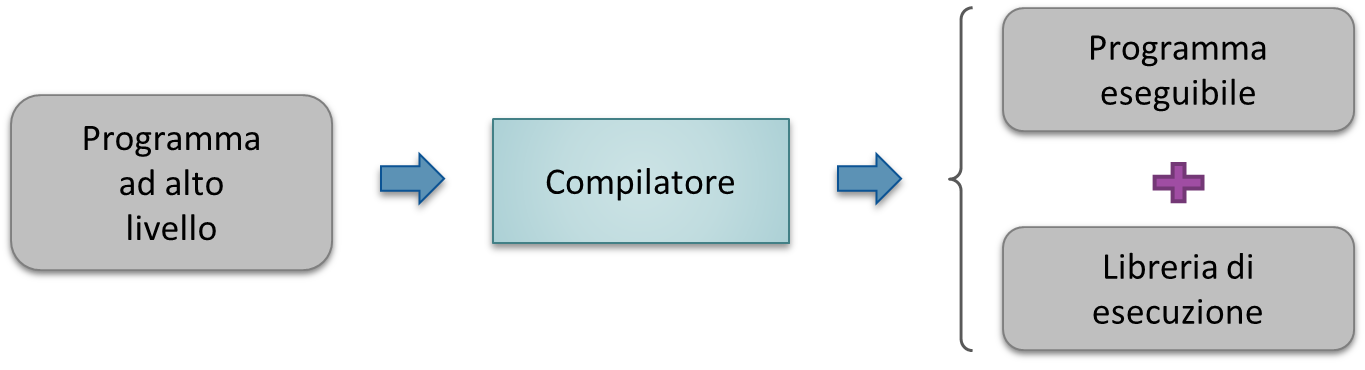
\includegraphics[width=0.75\linewidth]{images/API_Programming/Memoria/Memoria-esempio1.png}
\end{figure}

\section{Librerie di esecuzione}

Offrono agli applicativi meccanismi di base per il loro funzionamento
\begin{itemize}
    \item Supportano le astrazioni del linguaggio di programmazione 
    \item Forniscono un'interfaccia uniforme tra i diversi S.O. per le funzioni ad essi demandate 
\end{itemize}

Costituite da due tipi di funzioni 

\begin{itemize}
    \item Alcune, invisibili al programmatore, sono inserite in fase di compilazione per supportare l'esecuzione  (controllo dello stack, copia di aree di memoria ...)
    \item Altre offrono al programmatore funzionalità standard, gestendo opportune strutture dati ausiliarie e/o richiedendo al S.O. quelle non altrimenti realizzabili  (malloc o fopen)
\end{itemize}

\section{Modello di esecuzione nei linguaggi C e C++  }

In C/C++ sono pensati come se fossero gli unici utilizzatori di un elaboratore, completamente dedicato loro. Le uniche interazioni si riducono al più all'uso di risorse persistenti come il file system o le connessioni di rete .

L'isolamento è reso possibile dal meccanismo di indirizzamento virtuale.

Un programma C/C++ assume di poter accedere a qualsiasi indirizzo di memoria presente nello spazio di indirizzamento, all'interno del quale può leggere o scrivere dati o dal quale può eseguire codice macchina. Ma sappiamo che invece lo spazio di indirizzamento è:

\begin{itemize}
    \item Limitato
    \item Non contiguo
    \item Non tutto lo spazio consente ogni tipo di operazione 
\end{itemize}

\section{Esecuzione sequenziale sincrona, senza limitazioni  }

Un programma C/C++ è formato da un insieme di istruzioni eseguite, una per volta, nell'ordine indicato dal programmatore. 
Non ci sono limiti sul numero di istruzioni da eseguire, sul tempo richiesto alla loro esecuzione, né sulla memoria necessaria .

In realtà, tali limiti esistono e condizionano la scrittura dei programmi. Da qui nasce la necessità di un modello di gestione della memoria sicuro .

All'interno del flusso principale di esecuzione è possibile attivare flussi di elaborazione secondari, detti \textbf{thread}. Questi abilitano l'esecuzione concorrente (effettivamente parallela se la CPU è multicore) e introducono un ordine di grandezza nel livello di complessità della scrittura dei programmi. È il S.O. che si occupa di gestire tutti questi flussi di esecuzione indirizzandoli nei vari core fisici. 

\section{Flusso di esecuzione }

Il programma è costituito, come minimo, da un flusso di esecuzione il cui punto di partenza è predefinito:
\begin{itemize}
    \item La funzione main() nel linguaggio C
    \item I costruttori delle variabili globali in C++, seguiti dalla chiamata alla funzione main()
\end{itemize}

Vi sono inoltre due strutture dati:

\begin{itemize}
    \item Lo stack che permette permette di gestire chiamate annidate tra funzioni. Essa \textbf{supporta la ricorsione} e l'uso di \textbf{variabili locali}. In C++, supporta anche la gestione strutturata delle eccezioni
    \item Lo heap offre supporto per gestire dinamicamente l'utilizzo della memoria. Secondo logiche non strettamente correlate al procedere dell'esecuzione
\end{itemize}

\section{Stack}

Blocco di memoria allocato automaticamente all'avvio di un programma, circa 1 MB, al cui interno sarà possibile salvare:


\begin{itemize}
    \item Variabili locali e temporanee
    \item Gli argomenti passati ad ogni invocazione di funzione
    \item Valori di ritorno
    \item Traccia la storia delle chiamate a funzione
\end{itemize}

Viene utilizzato a partire da un estremo, espandendosi verso l'estremo opposto ogni volta che avviene una chiamata e contraendosi verso l'inizio quando una funzione ritorna.


Poiché ha dimensione finita, limita la profondità massima di ricorsione. Così come la dimensione totale delle variabili locali complessivamente utilizzabili.

Se, a seguito di un numero troppo elevato di chiamate o all'allocazione di variabili troppo grandi, si espande oltre il proprio limite, il sistema operativo (o il processore) interviene terminando l'esecuzione del programma generando un Stack overflow.\newline

\noindent
\begin{tcolorbox}
\textbf{Nota:} Stack = automatico, veloce, tempo di vita deterministico 
\end{tcolorbox}


\begin{center}
\begin{minipage}{0.85\linewidth}
  % Primo blocco: 50% dello spazio per il codice
  \begin{minipage}{0.55\linewidth}
\begin{minted}[breaklines]{c}
int f(int a) {
    int i = 5;
    if (a>0) {
        return a+i;
    } else {
        return a-1;
    }
}

int main() {
    int v = 9;
    v = f(v);
    return 0;
}        
\end{minted}
  \end{minipage}
  \begin{minipage}{0.40\linewidth}
      \centering
      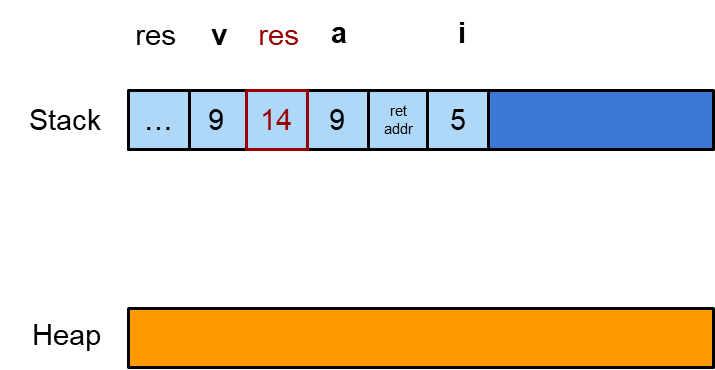
\includegraphics[width=1\linewidth]{images/API_Programming/Memoria/Memoria-esempio2.png}

      \vspace{0.2cm}

      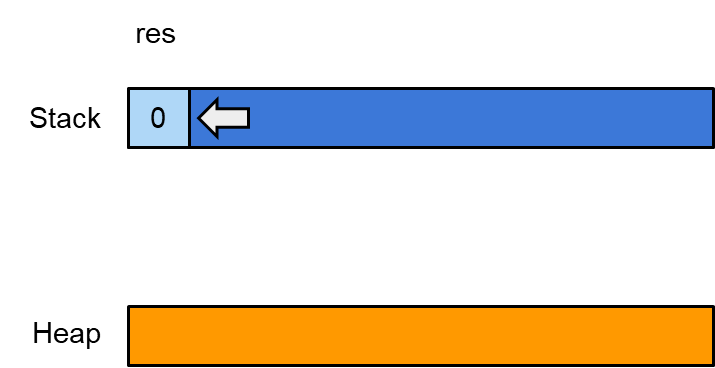
\includegraphics[width=1\linewidth]{images/API_Programming/Memoria/Memoria-esempio5.png}
      
  \end{minipage}
\end{minipage}
\end{center}

L'allocazione ed il rilascio sullo stack sono estremamente efficienti, grazie alla particolare politica di espansione / contrazione adottata.

Per contro, la durata dei valori memorizzati al suo interno è strettamente correlata alla durata dell'invocazione di un funzione. Non è possibile memorizzare nello stack un dato che duri più a lungo della funzione in cui è stato allocato. Per questo motivo, il chiamante di una funzione ha la responsabilità di pre-allocare lo spazio in cui dovrà essere memorizzato il risultato prodotto dalla funzione chiamata.


Inoltre, poiché lo spazio complessivo dello stack è definito a priori, non è possibile memorizzare un dato la cui dimensione superi tale spazio.
In generale, occorre limitare la dimensione massima del dato allocato ad una grandezza compatibile con il livello di profondità di chiamate e la dimensione degli altri dati che devono essere memorizzati complessivamente nello stack.  


\section{Heap}

Tutte le volte in cui un dato ha un ciclo di vita \textbf{non collegato al tempo di esecuzione} della funzione in cui è stato creato o la cui dimensione è \textbf{cospicua} oppure \textbf{non nota} in fase di compilazione, occorre richiederne la memorizzazione in una struttura a parte. I linguaggi C e C++ offrono un'apposita area, chiamata Heap o Free Store, all'interno della quale è possibile allocare e rilasciare blocchi di dimensione arbitraria (entro il limite della memoria disponibile).


A differenza di quanto avviene per lo stack, le aree allocate sullo heap non sono associate, a livello di linguaggio sorgente, ad un nome di variabile bensì si accede al loro contenuto esclusivamente tramite \textbf{puntatori}. Utilizzando l'operatore di dereferenziazione, *, posso accedere al contenuto memorizzato in memoria.

Questo spazio concesso dal S.O. è un prestito, dunque è responsabilità del programmatore rilasciare, prima o poi, la memoria allocata. Altrimenti si verificherà una perdita di memoria (memory leak) che, se reiterata, porta il sistema operativo a distruggere il processo.


\begin{center}
\begin{minipage}{0.85\linewidth}
  % Primo blocco: 50% dello spazio per il codice
  \begin{minipage}{0.55\linewidth}
\begin{minted}[breaklines]{c++}
int* f(int a) {
    if (a>0) {
        return new int[a];
    } else {
        return nullptr;
    }
}
int main() {
    int v = 2;
    int* buf = f(v);    //process buf
    delete[] buf;
    return 0;
}      
\end{minted}
  \end{minipage}
  \begin{minipage}{0.40\linewidth}
      \centering
      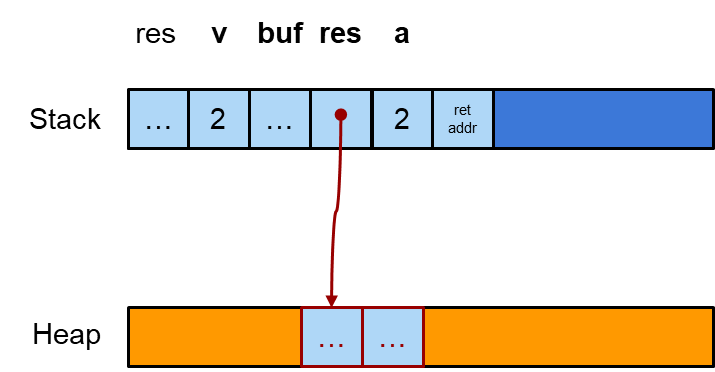
\includegraphics[width=1\linewidth]{images/API_Programming/Memoria/Memoria-esempio3.png}

      \vspace{0.2cm}
    
    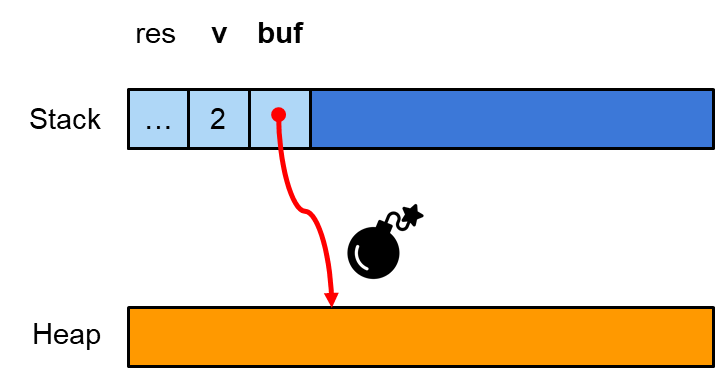
\includegraphics[width=1\linewidth]{images/API_Programming/Memoria/Memoria-esercizio4.png}
      
  \end{minipage}
\end{minipage}
\end{center}

Il puntatore è probabile che sia buono, ma non lo è, non gli è stato assegnato null, il linguaggio non te lo impone.

\section{Organizzazione dello spazio di indirizzamento  }

\begin{itemize}
    \item Codice eseguibile
        \begin{itemize}
            \item Contiene le istruzioni in codice macchina
            \item Accesso in lettura ed esecuzione
        \end{itemize}
    \item Costanti
         \begin{itemize}
            \item Accesso in sola lettura
         \end{itemize}
    \item Variabili globali
        \begin{itemize}
            \item Accesso lettura/scrittura
        \end{itemize}
    \item Stack
        \begin{itemize}
            \item Contiene indirizzi e valori di ritorno, parametri e variabili locali
            \item Accesso lettura/scrittura
        \end{itemize}
    \item Heap
        \begin{itemize}
            \item Insieme di blocchi di memoria disponibili per l'allocazione dinamica
            \item Gestiti tramite funzioni di libreria (malloc, new, free, …) che li frammentano e ricompattano in base
            \item alle richieste del programma
        \end{itemize}
\end{itemize}

Nel sistema operativo Linux, è facile verificare come sia organizzato lo spazio di indirizzamento di un programma in esecuzione (processo). Ogni processo è identificato univocamente da un numero intero (PID) e con il comando \textit{ps -ef} , il sistema operativo crea, per ciascun processo attivo, un file virtuale denominato \textit{/proc/<pid>/maps} che descrive lo spazio di indirizzamento con informazioni sui diversi segmenti al suo interno.

 
\section{Ciclo di vita delle variabili  }

Il modello di esecuzione dei linguaggi C/C++ distingue diverse tipologie di variabili 

\begin{center}
    Globali \qquad  locali \qquad  dinamiche 
\end{center}


Ciascuna classe ha un proprio ciclo di vita: Intervallo di tempo in cui è garantito l'accesso alle informazioni contenute al loro interno. 

\section{Variabili globali e locali  }

\begin{itemize}
    \item Le variabili globali hanno un indirizzo fisso, determinato dal compilatore e dal linker. Sono accessibili in ogni momento e all'avvio del programma, contengono l'eventuale \textbf{valore di inizializzazione}.
    \item Le variabili locali hanno un indirizzo relativo alla cima dello stack. Il ciclo di vita coincidente con quello della funzione/blocco in cui sono dichiarate. Il valore \textbf{iniziale è casuale}.
\end{itemize}

\section{Variabili dinamiche}

Le variabili dinamiche hanno un indirizzo assoluto, determinato in fase di esecuzione. Sono accessibili solo tramite puntatori, è il programmatore a controllarne il ciclo di vita e il valore iniziale può essere inizializzato o meno.


L'uso di questo tipo di variabili presuppone un'infrastruttura di supporto che offra meccanismi di allocazione e di rilascio fornita dalla libreria di esecuzione e dal S.O.  

\section{Allocazione della memoria  }

La libreria standard C offre vari meccanismi per ottenere l'indirizzo di un blocco allocato dinamicamente

\begin{minted}[breaklines]{c++}
void *malloc(size_t s)
void *calloc(int n, size_t s)   //per gli array
void *realloc(void* p, size_t s)   //rialloca aggiungendo memoria
\end{minted}

In caso di fallimento, viene restituito NULL, tranne nella \textit{realloc(...)} dove il blocco originale non viene toccato e il puntatore \textit{p} resta valido.\newline

In C++ viene definito il costrutto: \mintinline{c++}{new NomeTipo\{argomenti…\}  }

\section{Rilascio della memoria  }

Opportune funzioni di libreria permettono di restituire i blocchi precedentemente allocati.
Poiché ogni funzione di allocazione mantiene le proprie strutture dati, occorre che un blocco sia rilasciato dalla funzione duale di quella con cui è stato allocato:

\begin{itemize}
    \item \mintinline{c++}{malloc(…) / free(...)}
    \item \mintinline{c++}{new / delete}
    \item \mintinline{c++}{new ...[num\_elements] / delete[ ]}
\end{itemize}


Se il blocco non viene rilasciato si crea una perdita di memoria, che, a lungo andare, provoca l'esaurimento dello spazio di indirizzamento. 

Se il blocco viene rilasciato più volte o viene rilasciato con la funzione sbagliata si corrompono le strutture dati degli allocatori, con conseguenze imprevedibili.

\section{Puntatori}

Le variabili sullo heap possono essere gestite solo tramite puntatori perché la loro posizione non è nota a priori.

Vi è un problema, potentissimi per implementare di una vasta gamma di algoritmi come liste, grafo, etc., ma sono estremamente pericolosi. I puntatori sono intrinsecamente ambigui implica che il programmatore gestisca esplicitamente l'allocazione ed il rilascio dei blocchi al loro interno e ne manipoli il contenuto attraverso l'uso dei puntatori.

Il loro utilizzo espone infatti il programmatore ad una vasta gamma di errori, le cui conseguenze portano - nella maggior parte dei casi - a \textbf{comportamenti non definiti} (undefined behavior), le cui conseguenze sono disastrose.

\section{Il costo del rilascio}

I linguaggi gestiti, come Java, JavaScript, Python, C\#, etc.  gestiscono automaticamente il rilascio dei blocchi di memoria utilizzando il Garbage Collector. Per farlo, tengono traccia di chi punta a chi altro. Se, a partire dalle variabili presenti nello stack, un blocco non risulta più raggiungibile, questo può essere liberato. \newline

Per poter applicare questo algoritmo occorre "fermare il mondo". Ovvero \textbf{sospendere temporaneamente l'esecuzione del programma intero} per poter osservare una situazione statica e procedere con la compattazione dello heap. Questo può comportare lo spostamento di blocchi e il cambiamento del valore contenuto nei rispettivi puntatori.

L'operazione di rilascio può comportare pause non deterministiche. Talvolta incompatibili con contesti di esecuzione in tempo reale.

\section{Puntatori in C/C++}

Permettono l'accesso diretto ad un blocco di memoria, tale blocco può appartenere ad altri oggetti:

\begin{minted}[breaklines]{c++}
int A=10;
int* pA = &A;    
\end{minted}

o essere allocato allo scopo \mintinline{c++}{int* pB = new int{24}}

Possono essere esplicitamente resi invalidi:

\begin{itemize}
    \item Il valore \textit{0}
    \item La macro NULL$ \Rightarrow$\textit{((void *)0)}
    \item La parola-chiave \textit{nullptr}  (C++11 e superiori)
\end{itemize}

Quando si usano i puntatori, occorre stabilire quali responsabilità/permessi sono associati al loro uso.

\section{Le ambiguità dei puntatori in C/C++}

 \begin{itemize}
     \item Contiene un indirizzo valido?
     \item Quanto è grosso il blocco puntato?
     \item Fino a quando è garantito l'accesso?
     \item Se ne può modificare il contenuto?
     \item Occorre rilasciarlo?
     \item Lo si può rilasciare o altri conoscono lo stesso indirizzo?
     \item Viene usato come modo per esprimere l'opzionalità del dato?
 \end{itemize}



\noindent
\begin{tcolorbox}
\textbf{Nota:} In C/C++ il programmatore è responsabile; in Rust la responsabilità è codificata nel sistema dei tipi 
\end{tcolorbox}

\section{Problemi legati ai puntatori  }

In C, la gestione della memoria è totalmente affidata al programmatore 

\begin{itemize}
    \item Non ci sono supporti sintattici per automatizzare il ciclo di vita del blocco puntato
    \item Né meccanismi per associare una specifica semantica al puntatore
\end{itemize}

In C++ sono state introdotte nuove astrazioni (riferimenti, smart pointer) che sollevano il programmatore da alcune responsabilità, facilitando la creazione di programmi più robusti. Ma richiedono in ogni caso una comprensione approfondita del problema e l'uso attento e coerente dei puntatori.

\section{Responsabilità del programmatore  }

\begin{itemize}
    \item Limitare gli accessi ad un blocco
        \begin{itemize}
            \item Nello spazio: non accedere alle locazioni che lo precedono o che lo seguono
            \item Nel tempo: non accedere al blocco al di fuori del suo ciclo di vita
         \end{itemize}
    \item Non assegnare a puntatori valori che corrispondono ad indirizzi non mappati
         \begin{itemize}
            \item Possibile nel caso di cast o di assegnazione improprie
         \end{itemize}
    \item Rilasciare tutta la memoria dinamica allocata
         \begin{itemize}
            \item Una e una sola volta, usando la funzione duale di quella usata per la sua allocazione
         \end{itemize}
\end{itemize}


\section{Rischi }

Accedere ad un indirizzo quando il corrispondente ciclo di vita è terminato, ha
\textbf{effetti impredicibili}: 

\begin{itemize}
    \item Dangling pointer
    \item La memoria indirizzata può essere inutilizzata, in uso ad altre parti del programma o non mappata
\end{itemize}

Non rilasciare la memoria non più in uso, \textbf{spreca risorse} del sistema

\begin{itemize}
    \item Memory leakage
    \item Se si continua ad allocare senza mai rilasciare, si può saturare lo spazio di indirizzamento
\end{itemize}

Rilasciare la memoria più volte \textbf{corrompe le strutture} usate dallo heap, double free.\newline

Se si assegna ad un puntatore un indirizzo non mappato nello spazio di
indirizzamento e si usa quel puntatore, viene generata una interruzione del
processore. Il S.O. intercetta tale interruzione e termina il processo.


Se non si inizializza un puntatore e lo si usa, \textit{Wild pointer}, il suo contenuto potrebbe puntare
ovunque. Può causare una violazione di accesso oppure corrompere un'area di memoria in uso ad altre parti del programma.



\section{Problemi dei puntatori in C/C++  }

\begin{table}[H]
\renewcommand{\arraystretch}{1.6}
    \centering
    \begin{tabular}{l p{4.7cm}}
        % \hline
        \hline
        \textbf{Problema} & \textbf{Conseguenza} \\
        \hline
        dangling / wild pointer&  crash / UB\\
        double free&  corruzione heap\\
        leak & esaurimento della memoria\\
        data race & risultati casuali\\
       
        \hline
    \end{tabular}
\end{table}



\section{Le risposte di Rust  }

\begin{table}[H]
\renewcommand{\arraystretch}{1.6}
    \centering
    \begin{tabular}{l p{4.7cm}}
        % \hline
        \hline
        \textbf{Problema C / C++} & \textbf{Strumento Rust} \\
        \hline
        dangling / wild pointer&  borrow checker + tempo di vita\\
        double free&  gestione del possesso\\
        leak & pattern RAII\\
        nullptr & tipo Option<T>\\
        gestione del rilascio & tipi Box<T> / RC<T> / Arc<T>\\
       
        \hline
    \end{tabular}
\end{table}


\section{Gestire i puntatori  }

Chi alloca un blocco di memoria è \textbf{responsabile} di mettere in atto un meccanismo
che ne garantisca il successivo \textbf{rilascio}. Viene detto "possessore" del blocco.

Cosa capita se si effettua una copia di un puntatore?

Il secondo puntatore si trova coinvolto, suo malgrado, nel ciclo di vita del dato. Occorre introdurre un meccanismo per gestire efficacemente la semantica di un puntatore.


\section{Possesso della memoria  }

Il vincolo di rilascio risulta problematico per via dell'\textbf{ambiguità} del concetto di
puntatore all'interno del linguaggio. Dato un indirizzo non nullo, non è possibile distinguere se sia \textbf{valido o meno}, né \textbf{a quale area appartenga}, né se occorra o meno \textbf{rilasciarlo}.\newline

Ogni volta in cui si alloca un blocco dinamico e se ne salva l'indirizzo in una variabile
puntatore, quella variabile diventa proprietaria del blocco: ha la responsabilità di liberarlo.

Non tutti i puntatori posseggono il blocco a cui puntano. Se ad un puntatore viene assegnato l'indirizzo di un'altra variabile, la proprietà è della libreria di esecuzione.

Il problema si complica se un puntatore che possiede il proprio blocco viene copiato. Quale delle due copie è responsabile del rilascio?




\section{Dipendenze }


Quando si introducono strutture dati complesse, è comune che tali strutture
debbano appoggiarsi a blocchi di memoria ausiliari in cui memorizzare le
informazioni che esse gestiscono.

Un oggetto di tipo \mintinline{c++}{std::vector<T>}, in C++, incapsula un array dinamico di dati di tipo generico T:
tali dati possono essere aggiunti, rimossi, sostituiti, … tramite opportuni metodi sull'oggetto stesso. Tali blocchi ausiliari sono di proprietà dell'oggetto: vengono gestiti dai suoi metodi e devono essere
rilasciati quando l'oggetto viene distrutto.

Analogamente, altre strutture dati possono mantenere riferimenti a oggetti del
sistema operativo (handle a file, socket, timer, ...).Anche in questo caso le risorse corrispondenti risultano di proprietà dell'oggetto che le gestisce.


Collettivamente, questi tipi di dato prendono il nome di \textbf{dipendenze}.\newline

Il linguaggio C non offre nessun supporto sintattico per la gestione delle dipendenze
e lascia al programmatore la completa responsabilità della loro gestione


Al contrario, il linguaggio C++ offre, per gli oggetti di tipo \textit{class}, \textit{struct} e \textit{union} (!), la possibilità di specificare particolari funzioni membro dette rispettivamente costruttori e distruttori.

\begin{itemize}
    \item Un costruttore è una funzione membro che ha il compito di inizializzare un oggetto, provvedendo ad acquisire - se necessario - le sue dipendenze
    \item Il distruttore è una funzione membro che viene invocata automaticamente dal compilatore quando l'oggetto raggiunge la fine della propria esistenza ed ha il compito di rilasciare correttamente le dipendenze possedute dall'oggetto stesso
\end{itemize}



\section{Ma non basta scrivere un programma "giusto"?  }

Sì, basterebbe se fosse possibile essere certi che lo è! In realtà le cose sono molto più complesse.

Raramente i programmi sono scritti da una singola persona. Per lo più si appoggiano a librerie scritte da altri che hanno fatto opportune assunzioni su come debbano essere utilizzate, ma non è detto che tali assunzioni siano rispettate né, talvolta, conosciute. Spesso si lavora in gruppo e la comunicazione è imperfetta.

Al crescere della dimensione del programma, la quantità di particolari a cui occorre
badare cresce molto più in fretta. Ed è estremamente probabile dimenticarsi delle proprie assunzioni.



\section{Perché questo problema non si verifica in altri linguaggi?  }

Nella maggior parte dei linguaggi di alto livello il problema della gestione della
memoria non si pone, pur offrendo, a vario titolo, il concetto di puntatore.


Java, C\#, Python, JavaScript, …, basano il proprio meccanismo di rilascio su un
algoritmo di Garbage Collection. Libera il programmatore dalla responsabilità di rilasciare esplicitamente la memoria dinamica allocata, in cambio della perdita di controllo su \textbf{quando} e \textbf{come} tale rilascio avvenga.


La maggior parte di tali linguaggi basa la propria strategia di gestione della memoria
su una combinazione dei seguenti algoritmi:

\begin{itemize}
    \item Reference counting
    \item Mark and Sweep
\end{itemize}


\section{Confronto}

\begin{table}[H]
\renewcommand{\arraystretch}{1.6}
    \centering
    \begin{tabularx}{\textwidth}{X X}
        % \hline
        \hline
        \textbf{Gestione manuale in C/C++} & \textbf{Gestione automatica (Java/C\#/Python/Js)} \\
        \hline 
        Il rilascio avviene invocando la funzione \textbf{free()} o l'operatore \textbf{delete}& Il rilascio è eseguito automaticamente dal garbage collector\\
        
        Il momento in cui avviene il rilascio è controllato dal programmatore &  Il momento in cui avviene il rilascio è controllato dal garbage collector, che viene eseguito periodicamente \\
        
        In C++, gli oggetti dispongono di un distruttore che gestisce il rilascio esplicito delle dipendenze  &  Il concetto di distruttore non è parte del linguaggio (ecc. Java, con il metodo \textit{finalize()} ora deprecato) \\
        
        Il rilascio non comporta tempi supplementari di attesa, che sarebbero incompatibili con i sistemi in tempo reale   & Quando si attiva la garbage collection, il programma si arresta fino al termine dell'algoritmo, mettendo a rischio il funzionamento di un sistema in tempo reale\\
        
        Si possono verificare memory leak, doppi rilasci, dangling pointer, wild pointer & Non possono verificarsi errori sulla gestione della memoria\\
    \end{tabularx}
\end{table}

